\chapter{系统运行观测}

CoTriage 的价值不只在于把日志送入不同模型，而在于能否在现场时限、诊断质量、云端开销和异常网络之间取得可解释的平衡。因此，本章围绕五个可验证问题组织观测指标：边缘侧能否及时给出首个可用判断；按需上云能否在保留诊断能力的同时减少传输和调用；云端是否真正补充了跨节点上下文与处置知识；外部服务不可用时实时主链能否继续工作；节点和日志来源增加后，协同链路是否仍保持统一。
观测指标运行支持系统用户确认组件状态、事件流量、路由分布、队列积压和单事件追踪。

\begin{table}[htbp]
  \centering
  \small
  \caption{CoTriage 的核心评估问题、测量量与证据来源}
  \label{tab:evaluation-framework}
  \begin{tabularx}{\textwidth}{>{\bfseries}p{0.17\textwidth} p{0.29\textwidth} p{0.25\textwidth} X}
    \toprule
    评估问题 & 关键测量量 & 推荐对照 & 证据来源 \\
    \midrule
    现场响应能力 & 首次可用判断 P50／P95、边缘处理时延、吞吐率 & 仅边缘、全部上云、固定阈值级联 & 事件时间戳与压测记录 \\
    感知与决策质量 & Accuracy、Macro-F1、高风险 Recall、任务完成率 & 各边缘层级及云边协同策略 & 冻结并标注的数据集 \\
    协同与通信效率 & 本地闭环率、上云比例、上传字节、Token／事件、云端调用次数 & 全量上云与固定级联 & 路由记录、网关用量和流量统计 \\
    弱网运行韧性 & 本地业务保持率、Defer 数量、Outbox 峰值、重放成功率与排空时间 & 正常、时延、丢包、断连和恢复窗口 & 故障注入记录与 Outbox 状态迁移 \\
    多节点适应性 & 节点数—吞吐曲线、端到端时延波动、相关事件冲突与收敛结果 & 不同节点规模和日志来源组合 & 设备登记、关联任务与决策审计 \\
    \bottomrule
  \end{tabularx}
\end{table}

一次事件处理包含采集、事件化、边缘推理、路由决策、可选的云端诊断以及反馈写回。由于云端诊断采用异步增强模式，系统区分“首次可用判断时延”和“完整诊断时延”：前者从采集时间起算，到边缘结果可被业务侧读取为止；后者在需要上云时继续计时，直到结构化诊断写回。这样的划分能够反映 CoTriage 的真实交付方式，也避免用较慢的云端完整生成掩盖边缘早期判断的价值。

\begin{figure}[htbp]
  \centering
  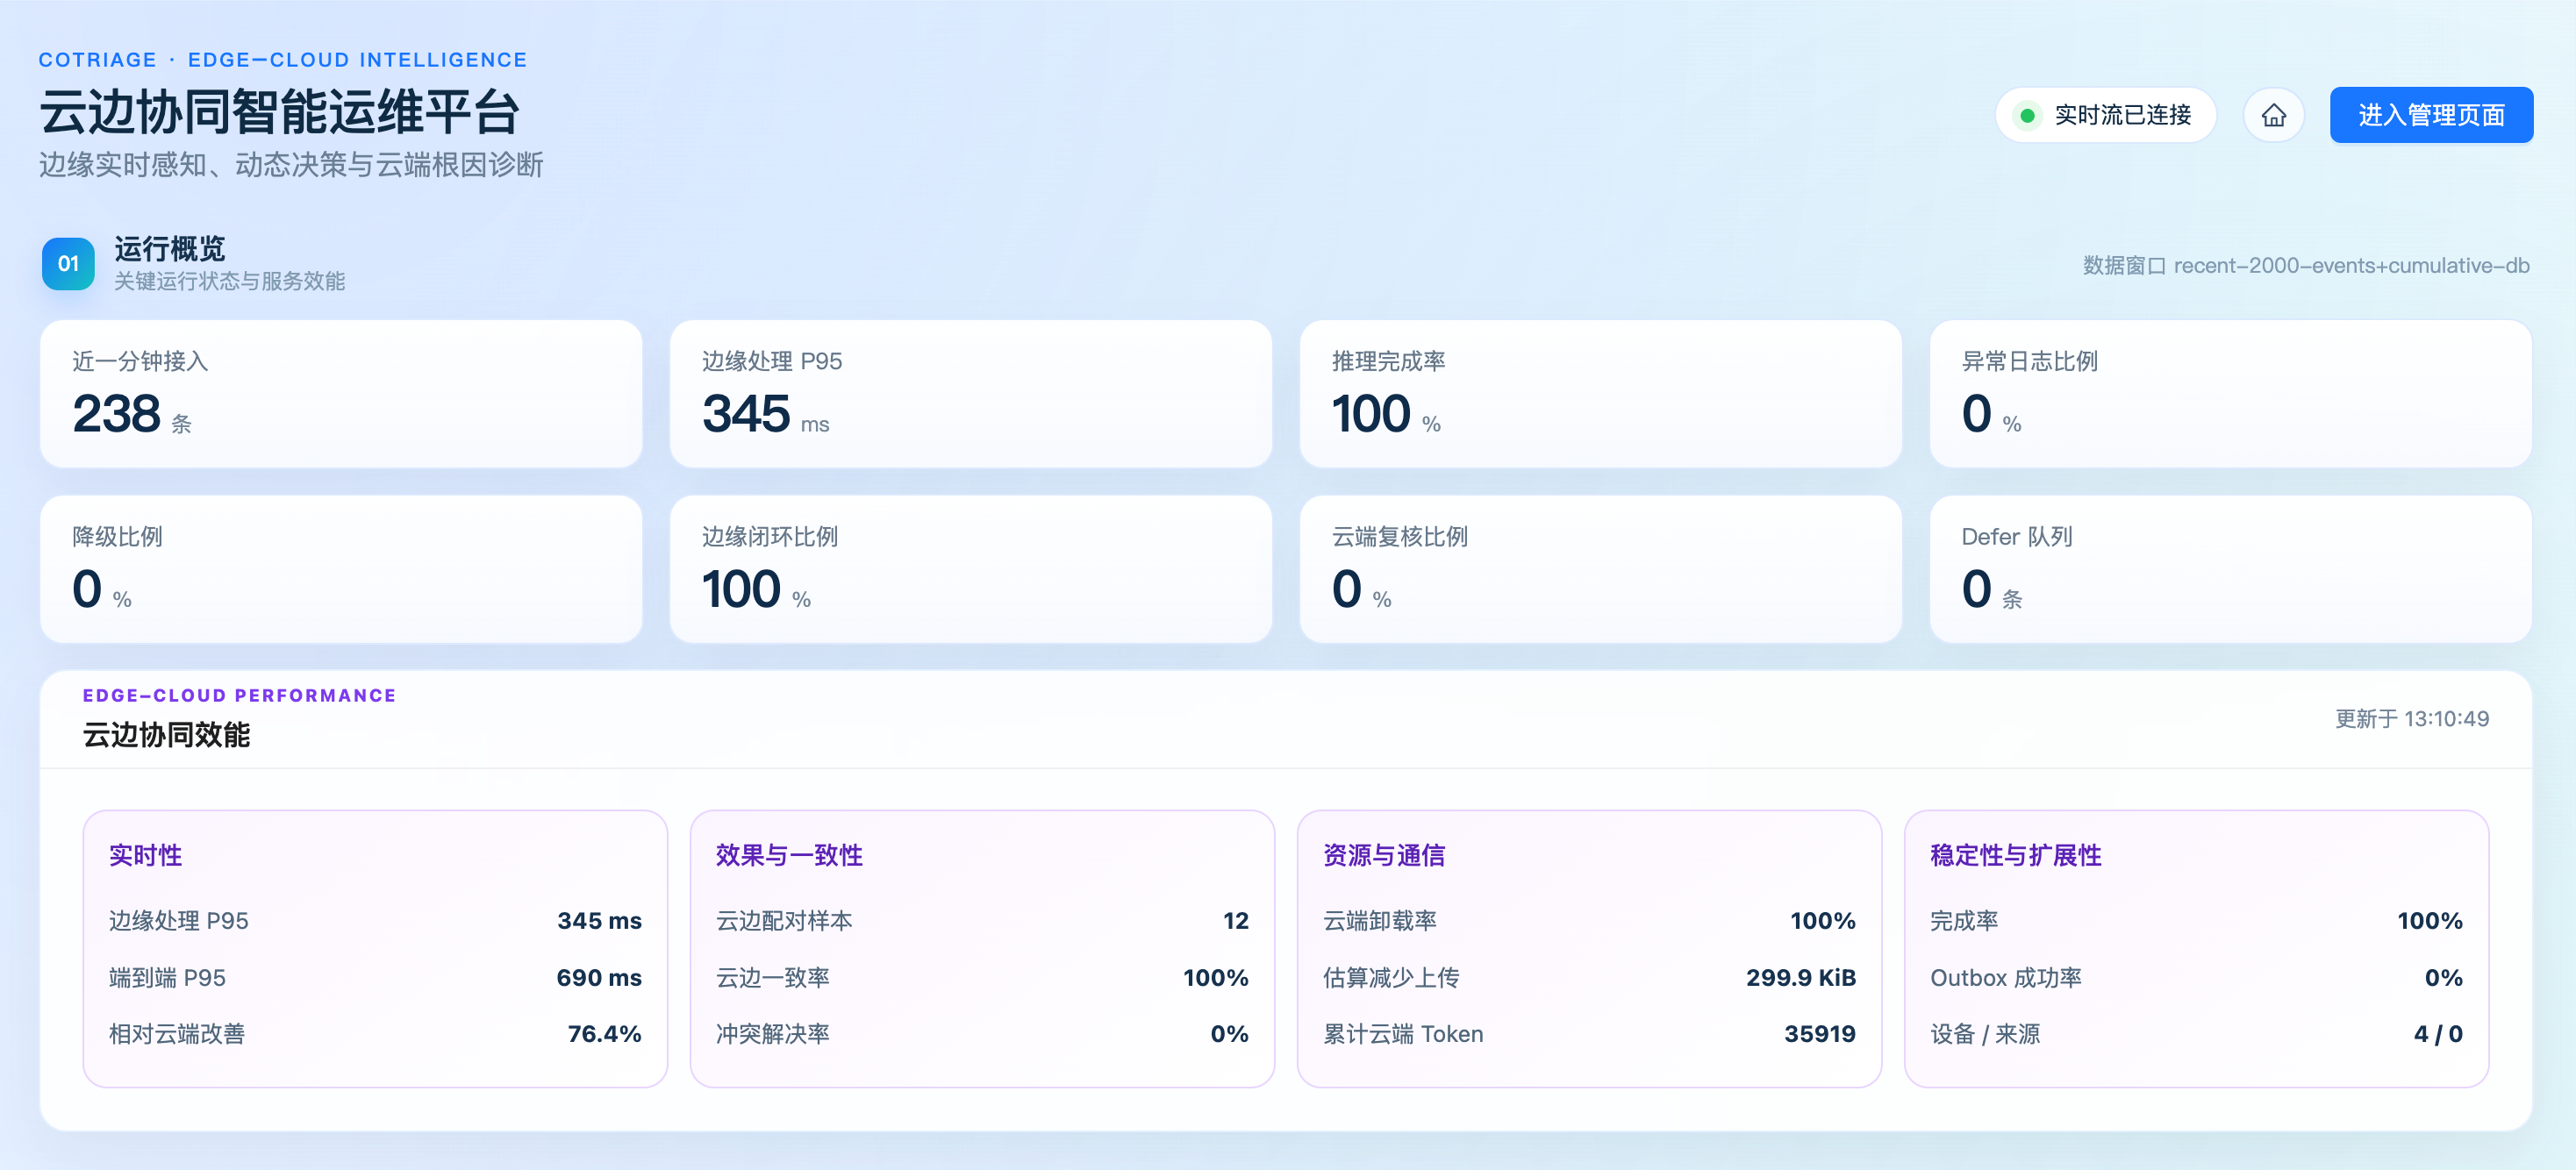
\includegraphics[width=\textwidth]{figures/s-11-competition-metrics-dashboard.png}
  \caption{CoTriage 运行质量分析界面：时延、路由、通信与可靠传输状态}
  \label{fig:runtime-quality-dashboard}
\end{figure}

\cref{fig:runtime-quality-dashboard}把接入、边缘处理、推理完成、异常、降级、云端复核和 Defer 状态组织在同一页面中，并进一步展示处理时延、边云配对、上传量、Token、Outbox 和节点接入情况。它的主要作用是把一次系统运行拆解成可追踪的阶段：运维人员既能看到总体负载与分流结构，也能沿事件标识下钻到推理路径、路由动作、云端请求和最终诊断。